%!TEX root = ../scivis_lbaakman_bvanloon.tex
\chapter{Glyphs} % (fold)
\label{cha:glyphs}
In this chapter a set of \emph{Glyphs} is introduced. Glyphs is a visualization technique which can be used to visualize a vector field by showing its orientation and magnitude. This is done by using icons that show direction and magnitude. A disadvantage of glyphs is the size the icons take in; because icons need to show both direction and magnitude they need to be of some size to convey this information in a clear matter. This means that the number of glyphs used in the visualization needs to be restricted to avoid clutter and glyphs blending together. This means the visualization can not be as `dense' as the scalar visualization meaning that not for every point of the simulation information can be shown. In the next section we discuss how the simulation is (sub)sampled and how we prevent the glyphs from cluttering used a grid and proper scaling. In \cref{sec:types_of_glyps} the different glyphs are discussed that we have chosen to implement.

\section{Method} % (fold)
\label{sec:method}
The main method for constructing glyphs is to sample the dataset and place a glyph at every sample-point. This glyphs is than scaled, colored and rotated based on the values on this sample-points. 

\subsection{Visualization Grid} % (fold)
\label{sub:sampling_grid}
Since glyphs can not be shown for every vertex of the simulation due to there size, we need to (sub)sample the simulation using sampling points. The number of sampling points denotes how many glyphs are shown. Less sampling points will result in less glyphs and thus less clutter, but also lessens the amount of information that is displayed. Increasing the number of sampling points size will increase the amount of information in the visualization, but might increase cluttering which can interfere with how well the information can be understand by the user. 

To facilitate the sampling a visualization grid is constructed\footnote{Note that the visualization grid is also used in combination with other visualization methods, but since the glyph visualization is the first technique in which the grid is used, it is introduced in this chapter.}.  The grid is defined on top of the simulation grid, ensuring the simulation is uniformly covered. Each vertex of the visualization grid is contained within the simulation grid and has a reference to the cell in the simulation grid that encloses the vertex. When data is requested from the visualization grid, for all sampling points on the visualization grid the values are calculated using bilinear interpolation of the vertices of its containing cell. 

Given a cell C with vertices containing some scalar value denoted by up left $(C_{UL})$, up right $(C_{UR})$, bottom left $(C_{BL})$, and bottom right $(C_{BR})$, these scalar values are bilinear interpolated for a point $p$ using the following rule:
\begin{align*}
	s & = C_{UL} * (1 - p_x ) * (1 - p_y) \\
		& +	C_{UR} *  p_x  * (1 - p_y) \\
		& +	C_{BL} *  (1 - p_x ) * p_y \\
		& +	C_{BR} *  p_x  * p_y. \\
\end{align*}
Vector data is interpolated by bilinear interpolations of the single components. Since it is unlikely to find inflection points between the sampled points of our vector fields, if the used sampling grid has a high enough density, we find bilinear interpolation of the elements of the vectors sufficient


\subsubsection{Jitter} % (fold)
\label{ssub:jitter}
When glyphs are shown on a uniform grid artifacts might appear when the sampling rate causes non existing patterns to appear in the visualization. These patterns can be avoided by adding some random shifts in the sampling grid. This is done by shifting each grid-point by a random factor controlled by the jitter factor. This way the grid stays a structured grid since the order of the vertices does not change, but the grid will no longer be uniform which prevents the appearance of artifacts. In \cref{fig:jitter} the effect of adding jitter is shown, the visualization that uses a grid without jitter in \cref{fig:jitter:nojitter} contains artificial patterns, while \cref{fig:jitter:jitter} does not.
\begin{figure}[tbh]
	\centering
	\begin{subfigure}{0.45\textwidth}
		\centering
		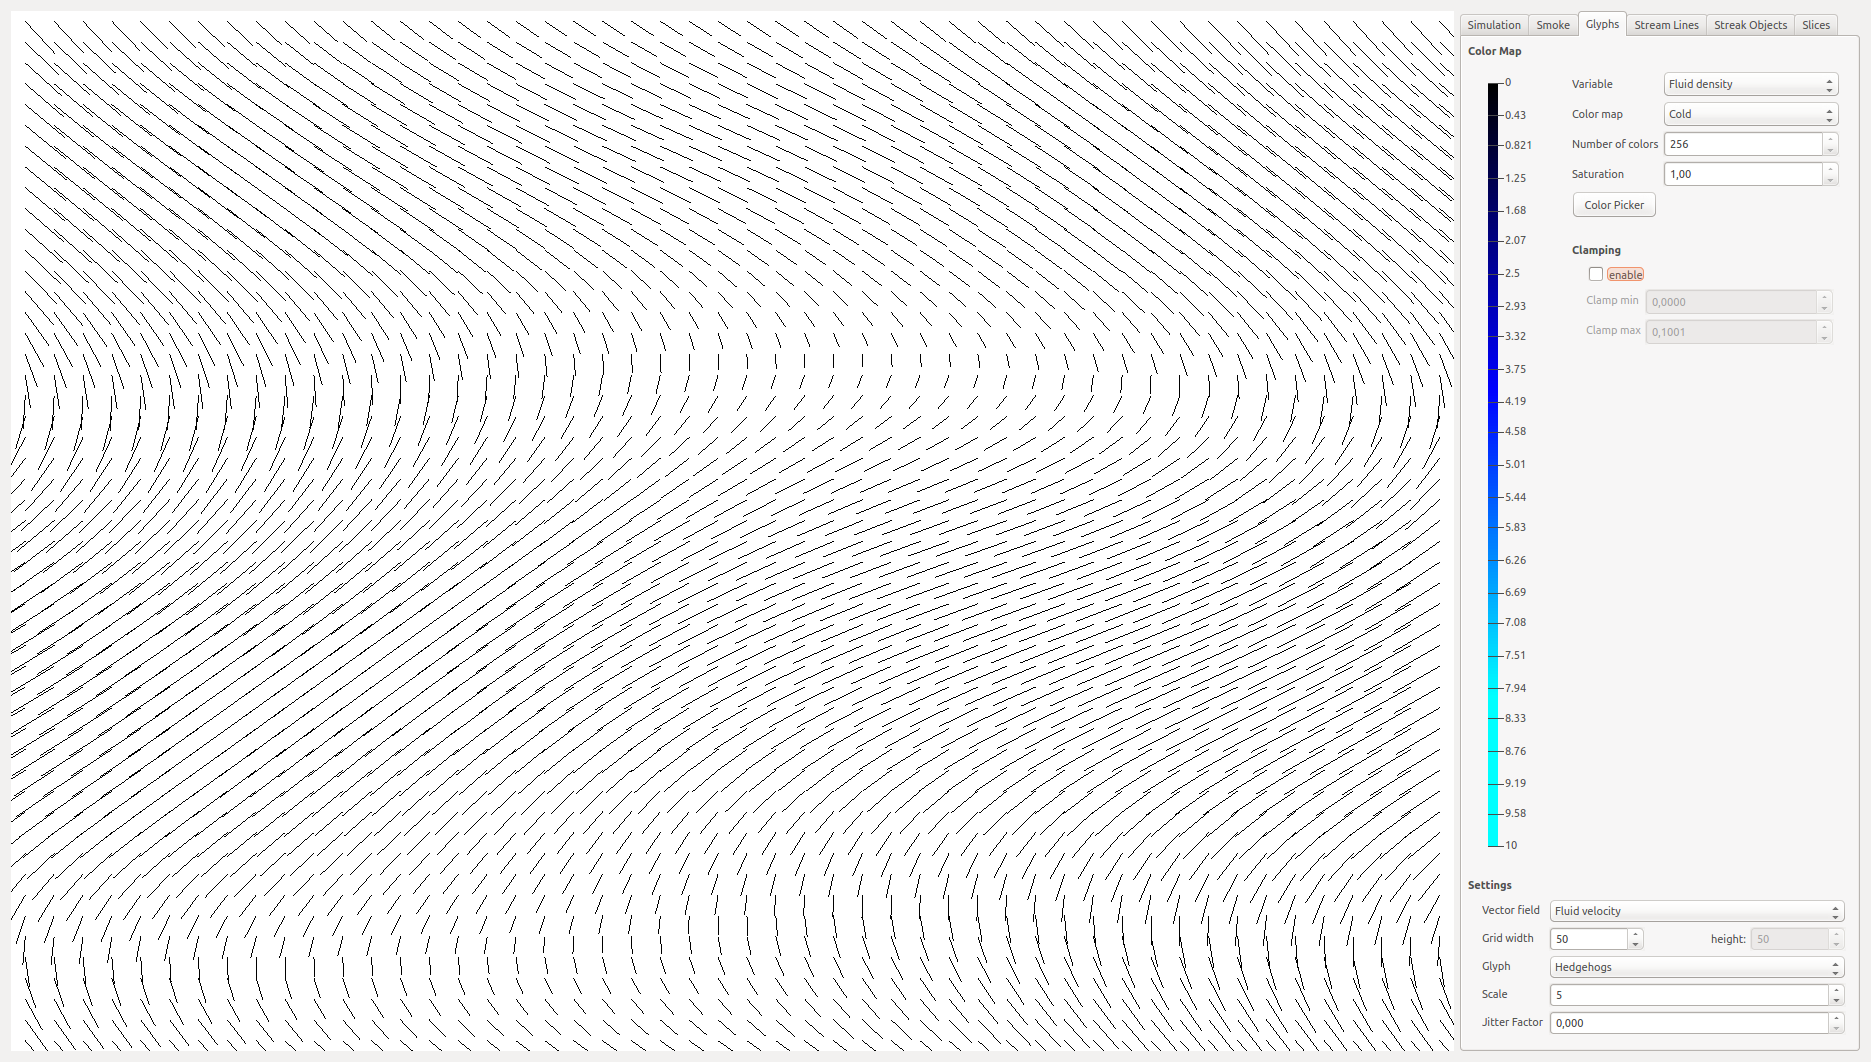
\includegraphics[width=0.9\textwidth, trim={35px 30px 430px 30px}, clip]{img/glyphs/nojitter}
		\caption{Vector visualization of the fluid velocity without jitter.}
		\label{fig:jitter:nojitter}
	\end{subfigure}
	\hspace{30px}
	\begin{subfigure}{0.45\textwidth}	
		\centering
		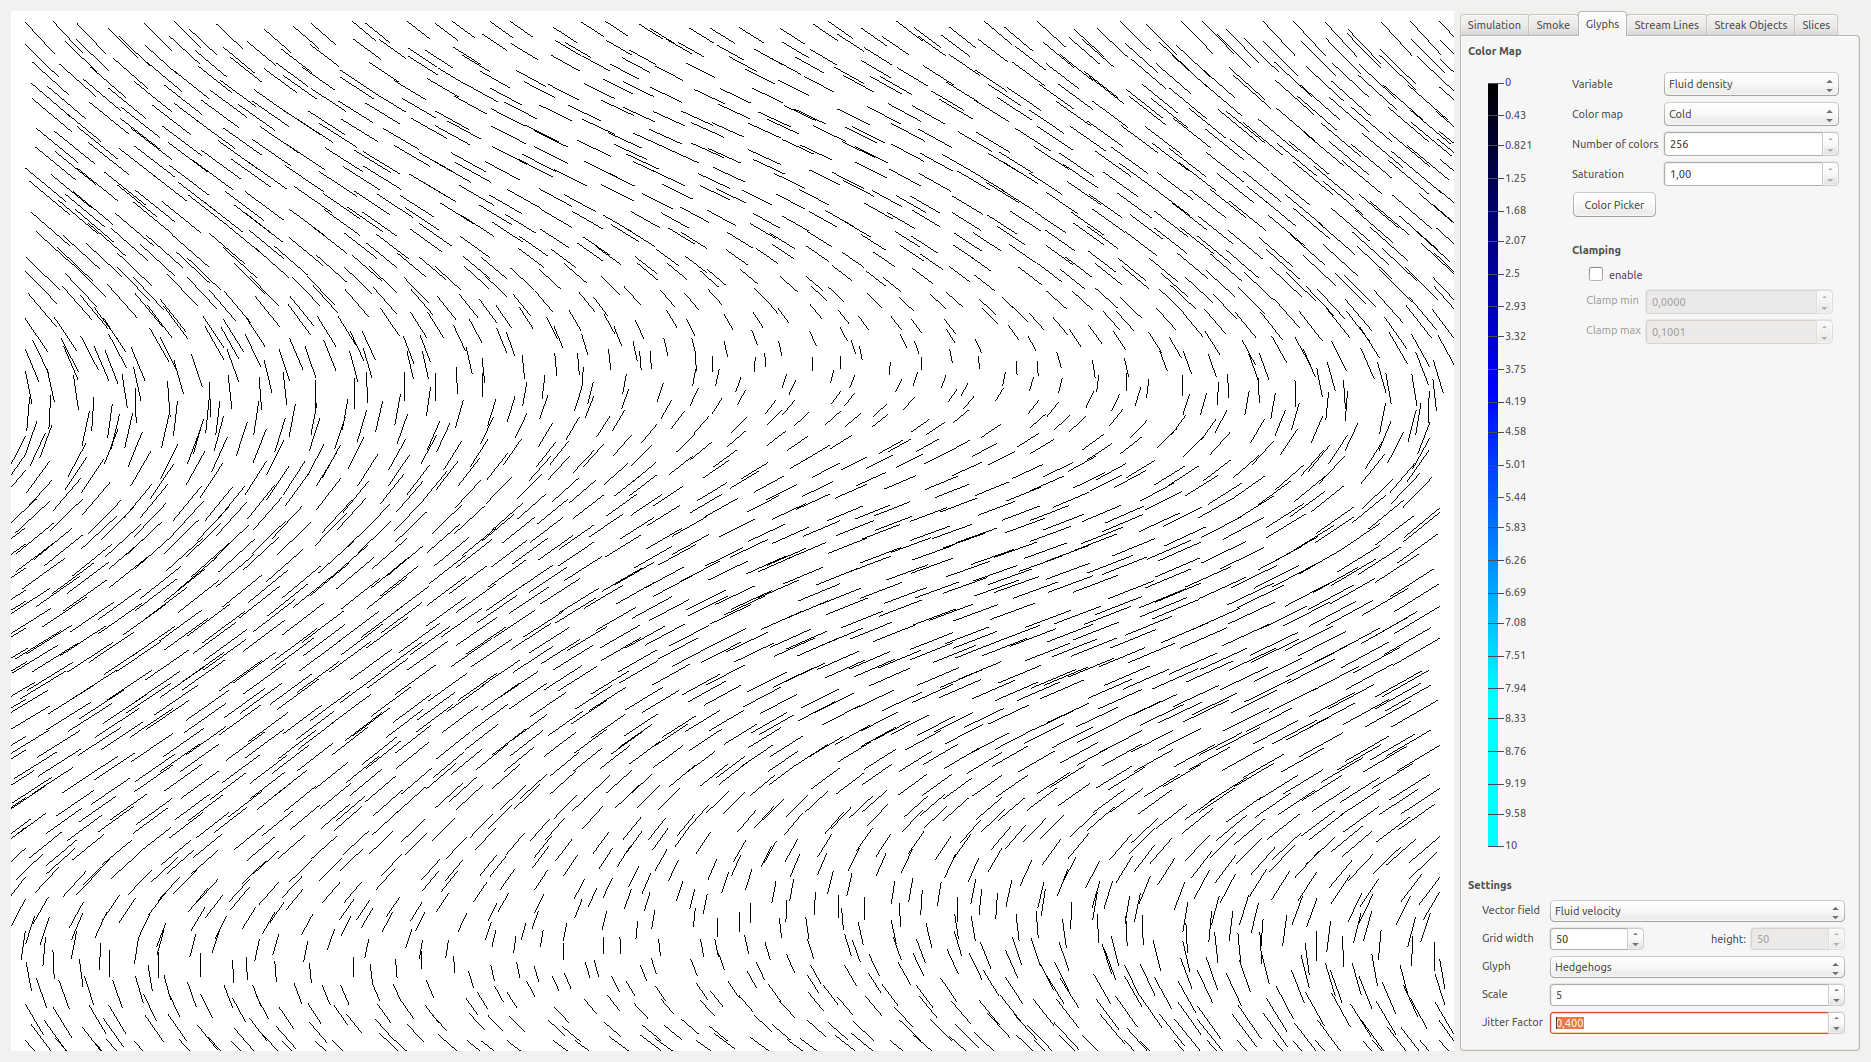
\includegraphics[width=0.9\textwidth, trim={35px 30px 430px 30px}, clip]{img/glyphs/jitter_0.4}
		\caption{Vector visualization of the fluid velocity with a jitter-factor of 0.4.}
		\label{fig:jitter:jitter}
	\end{subfigure}
	\caption{The effect of adding jitter to the vector visualization using hedgehogs. In \subref{fig:jitter:nojitter} clear patterns and artifacts are visible while this is not the case in \subref{fig:jitter:jitter}.}
	\label{fig:jitter}
\end{figure}

\subsection{Scaling} % (fold)
\label{sub:scaling}
In vector visualization glyphs are scaled to show the magnitude of the vector. In our application the size of the glyph is scaled relative to the size of its containing cell. This is done to prevent glyphs from becoming too large which causes cluttering, another advantage is that glyphs will take up more space when the cell size increases, making optimal use of the available space. To ensure the scaling of the glyphs is linear there is no minimum size of the glyph required. This has as disadvantage that glyphs of vectors with a very small magnitude might not be visible, but makes for a more natural ordered magnitude. The scaling can also be tweaked using a scale-factor which can be set by the user.
\begin{figure}[tbh]
	\centering
	\begin{subfigure}{0.45\textwidth}
		\centering
		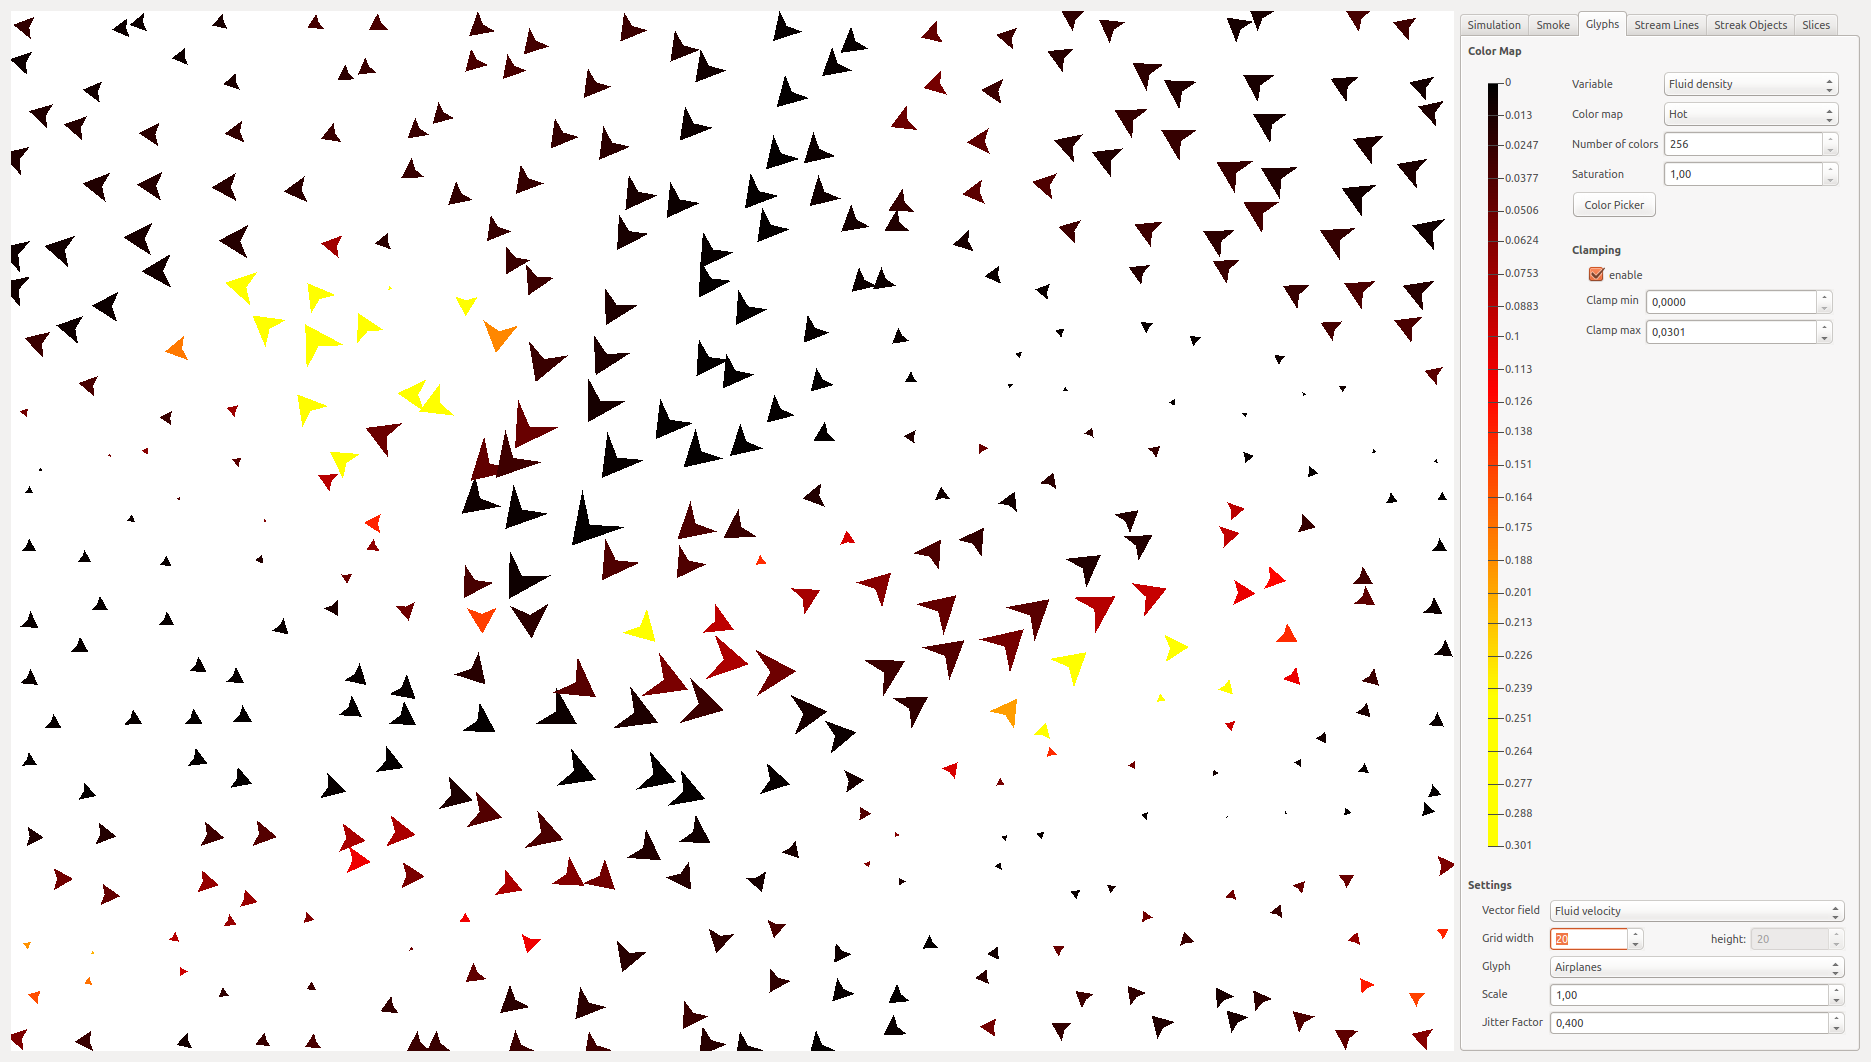
\includegraphics[width=0.9\textwidth, trim={35px 30px 430px 30px}, clip]{img/glyphs/scaling_20}
		\caption{Vector visualization of the fluid velocity using airplane glyphs on a 20x20 grid.}
		\label{fig:scaling:20}
	\end{subfigure}
	\hspace{30px}
	\begin{subfigure}{0.45\textwidth}	
		\centering
		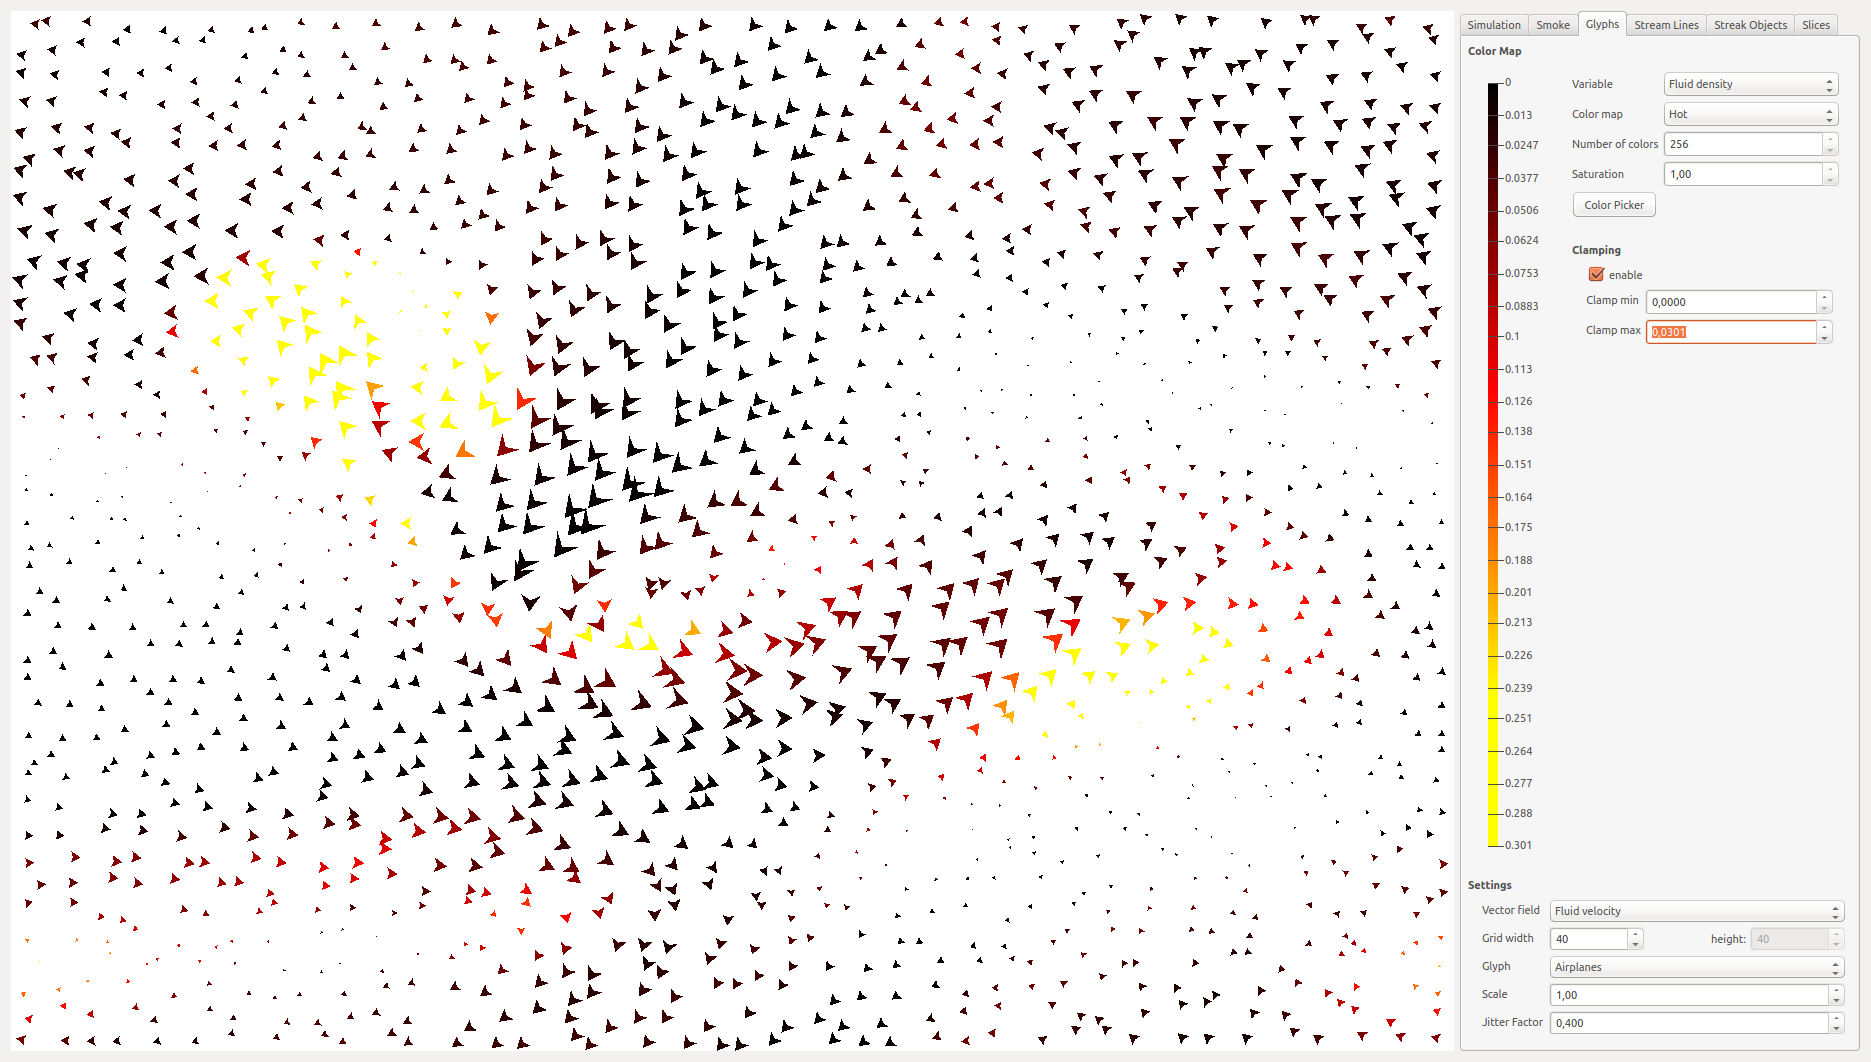
\includegraphics[width=0.9\textwidth, trim={35px 30px 430px 30px}, clip]{img/glyphs/scaling_40}
		\caption{Vector visualization of the fluid velocity using airplane glyphs on a 40x40 grid.}
		\label{fig:scaling:40}
	\end{subfigure}
	\caption{In this figure the same simulation is shown twice using airplane glyphs on grids of different sizes. When comparing \subref{fig:scaling:20} with \subref{fig:scaling:40} we can how the size of the glyph changes to avoid clutter while still using as much space as possible. }
	\label{fig:scaling}
\end{figure}

% section method (end)



\section{Types of Glyps} % (fold)
\label{sec:types_of_glyps}
In this section the glyphs implemented in the application are given. Each glyph is accompanied by a short discussion given its strong and weak points.
\subsection{Hedgehogs} % (fold)
\label{sub:hedgehogs}
The simplest form of glyphs are hedgehogs. Hedgehogs are lines which are placed in the direction of the vector and stretched relative to its magnitude. The glyph can be colored in two ways, first we can let the color of the glyph correspond with the vector magnitude. This way the magnitude is conveyed to the user by both the length and the color of the glyph which can help inverse mapping. Alternatively the glyph can be colored according to some scalar value. This increases the information density of the visualization, but might damper the clarity of the visualization.

Hedgehogs have as advantage that the glyph takes up relatively little space. A major drawback of hedgehogs is that it is not possible to distinguish two vectors going in opposite directions, as they will be represented by the same line. 

\subsection{Triangles} % (fold)
\label{sub:triangles}
The triangle glyph is one of the simplest glyphs that can give directional information. It is constructed by placing the middle of one side of the triangle orthogonal on the vector. The two others sides are stretched in the direction of the vector relative to the vectors magnitude. Thus, the triangle will appear longer as the magnitude of the vector increases. Besides the length the surface of the triangle also increases, which will help the inverse mapping process from glyphs back to magnitudes.

Although the triangles properly conveys the direction in most cases, a problem arises when the magnitude scales the triangles such that the extended sides become as long as the base side.  When this happens the triangle becomes equilateral and can no longer be mapped to a single direction, but corresponds to three different directions. This could be solved by curving the two extended sides inwards or by making the triangle into an arrow. Unfortunately these solutions are not implemented in the application. 

The triangle glyph is implemented such that the base side has a fixed length. This has as side-effect that vectors with a small magnitude might appear as lines orthogonal to the vector field. This can confuse users not aware of this effect, who therefore might interpret the triangle as a hedgehog. This increases the learning curve of the visualization but does not have to be a problem once the user is aware.

\subsection{Airplanes} % (fold)
\label{sub:airplanes}
In the previous section two flaws of the triangle where pointed out that could cause possible difficulty with the inverse mapping process. These flaws are fixed by the airplane glyph discussed in this section. The airplane glyph is a 3D glyph that exist out of two mirrored triangles joined by one side forming an airplane like structure. Depending on the vector magnitude the sides joined together will be pulled upwards, while the free vertex of both triangles will be pulled backwards. This has as effect that the airplane will become longer and pointier as the magnitude increases. Therefore the larger the magnitude becomes, the more prominent the direction of the glyph will be. This has two positive effects. Increasing magnitudes will have a clear natural order and as the magnitude increases the direction of the glyph becomes better visible. Since one can argue that the direction of a vector is of more importance when its magnitude increases this can be seen as a positive effect.

Since the airplane is a 3D glyph it is possible to use shading with the glyph visualization. This means that in the case of overlapping glyphs, single glyphs can be distinguished more easily due to the visual clues shading offers. 

The airplane glyph has a drawback concerning its scaling. When an airplane glyph is scaled up based on some magnitude, its wings are pushed down and its base is pulled up. Because the perspective in which the glyphs are shown (top-down) is not orthogonal to the glyphs surface, the `wings' of the glyph become skewed, meaning that the visible surface of a glyph is smaller than its real surface. This effects increases as the glyph is scaled up, meaning that its relative surface becomes smaller as its corresponding magnitude increases which means the ordering of the magnitude becomes non-linear. Because of this (possible harmful) effect the inverse mapping from glyph surface to magnitude becomes a bit more difficult for larger magnitudes.
% subsection airplanes (end)


\subsection{Results} % (fold)
\label{sec:results}
In this section visualizations are shown based on the same simulation using the three types of glyphs.
\begin{figure}[tb]
	\centering
	\begin{subfigure}{0.6\textwidth}
	\centering
	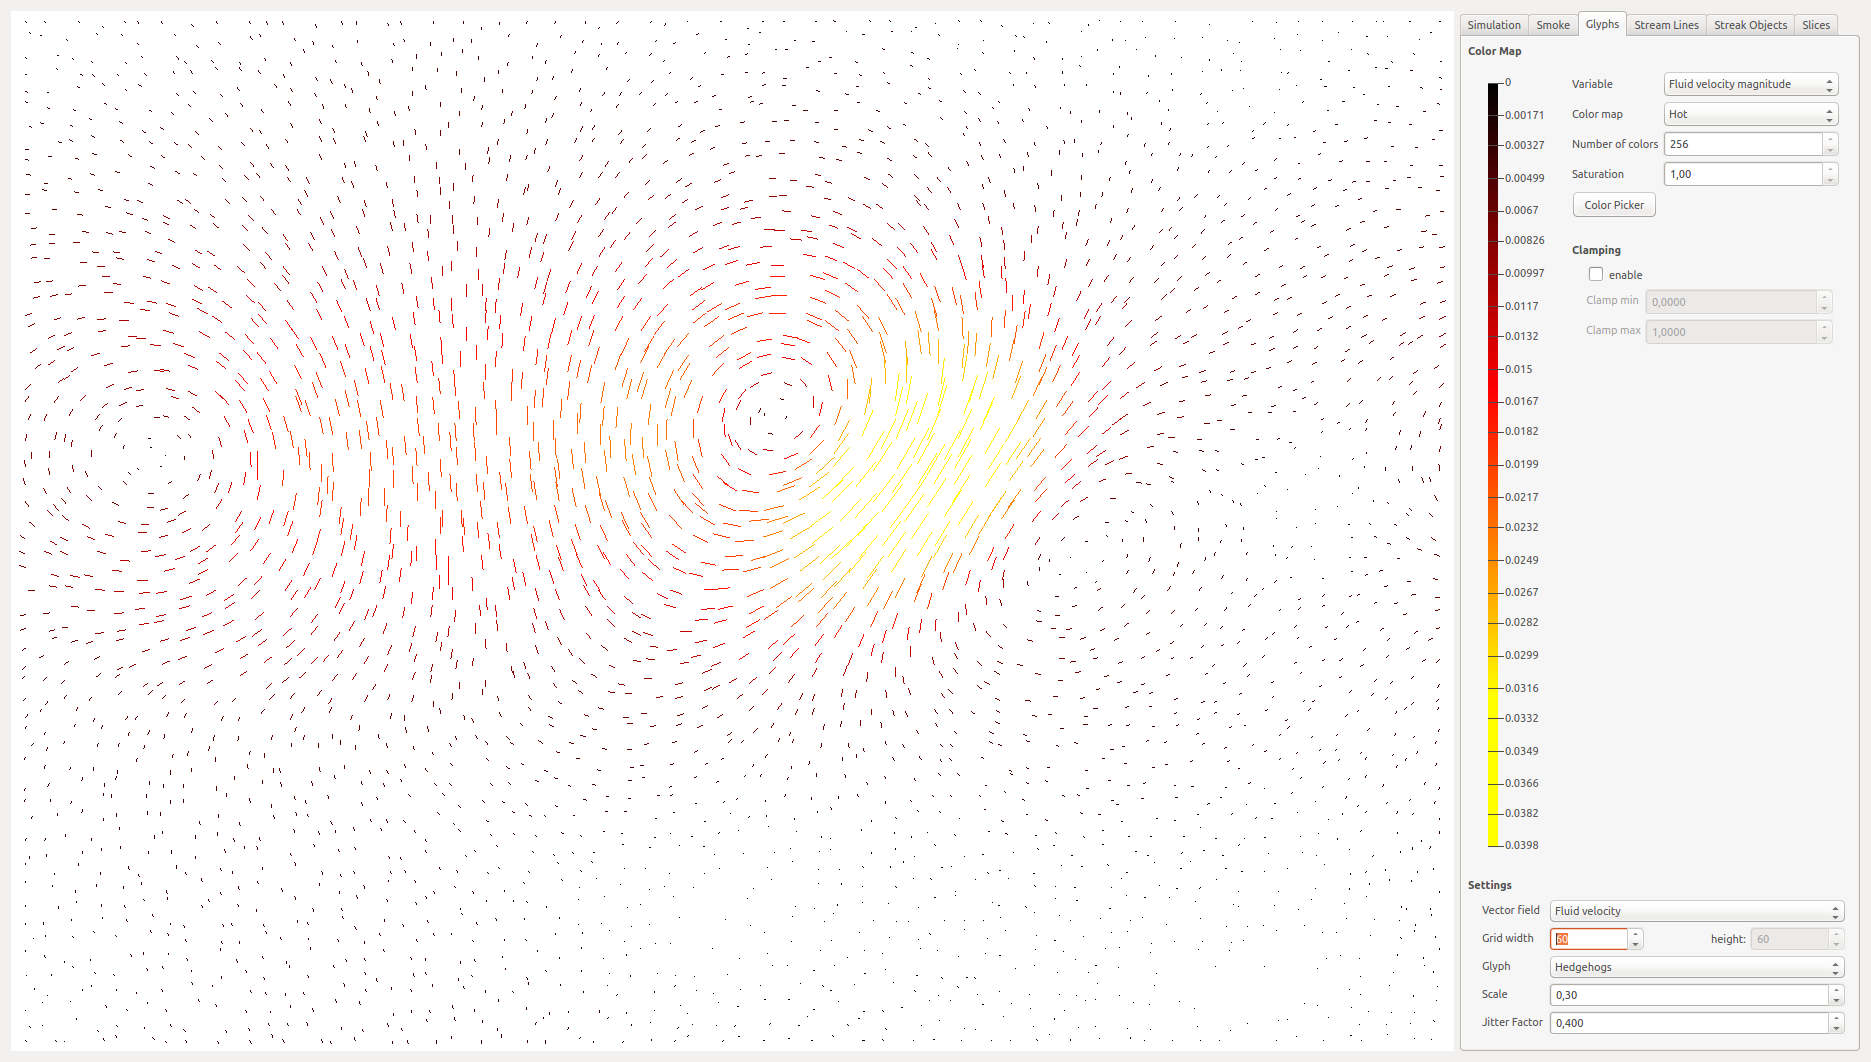
\includegraphics[width=\textwidth, trim={35px 30px 430px 30px},clip]{img/glyphs/hedgehogs.png}
	\caption{Example of hedgehogs showing the fluid velocity on a 60x60 grid.}
	\label{fig:glyphs:hedgehogs}
	\end{subfigure}
	\begin{subfigure}{0.6\textwidth}
		\centering
		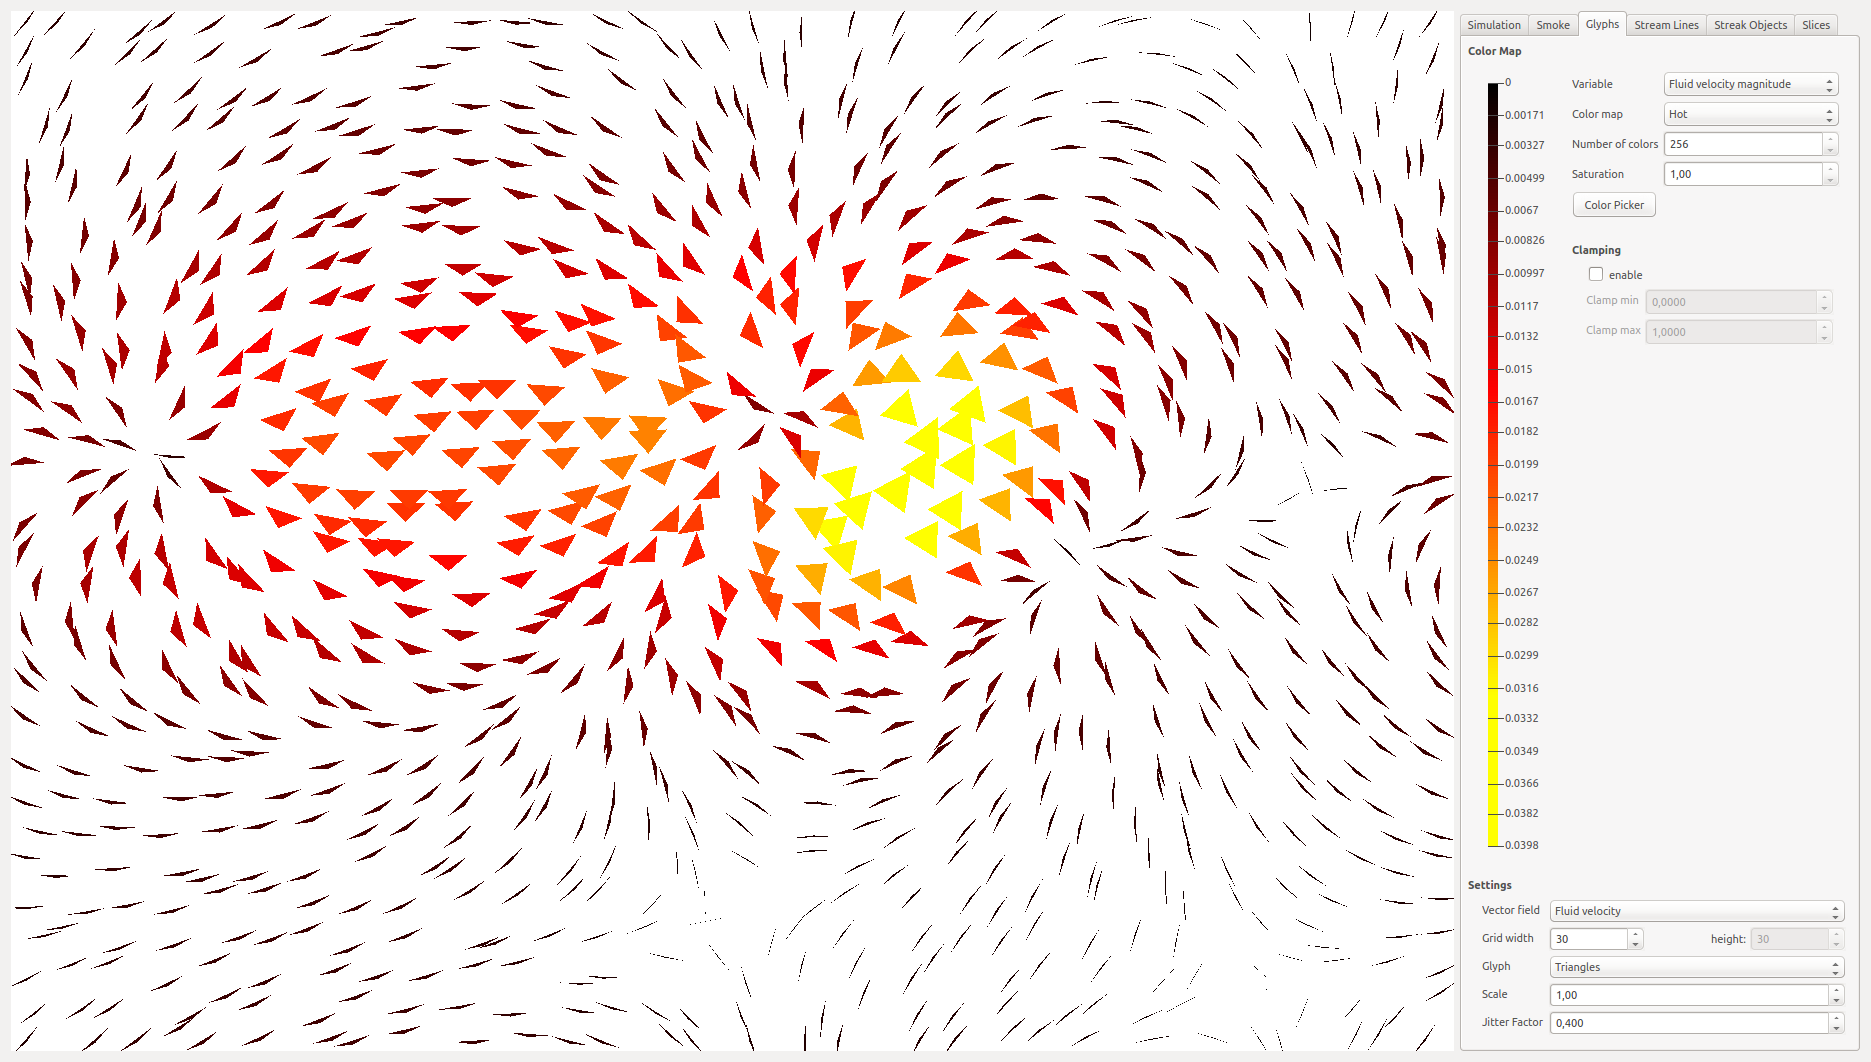
\includegraphics[width=\textwidth, trim={35px 30px 430px 30px},clip]{img/glyphs/triangles.png}
		\caption{Example of triangle glyphs showing the fluid velocity on a 30x30 grid.}
		\label{fig:glyphs:triangles}
	\end{subfigure}
	\begin{subfigure}{0.6\textwidth}
		\centering
		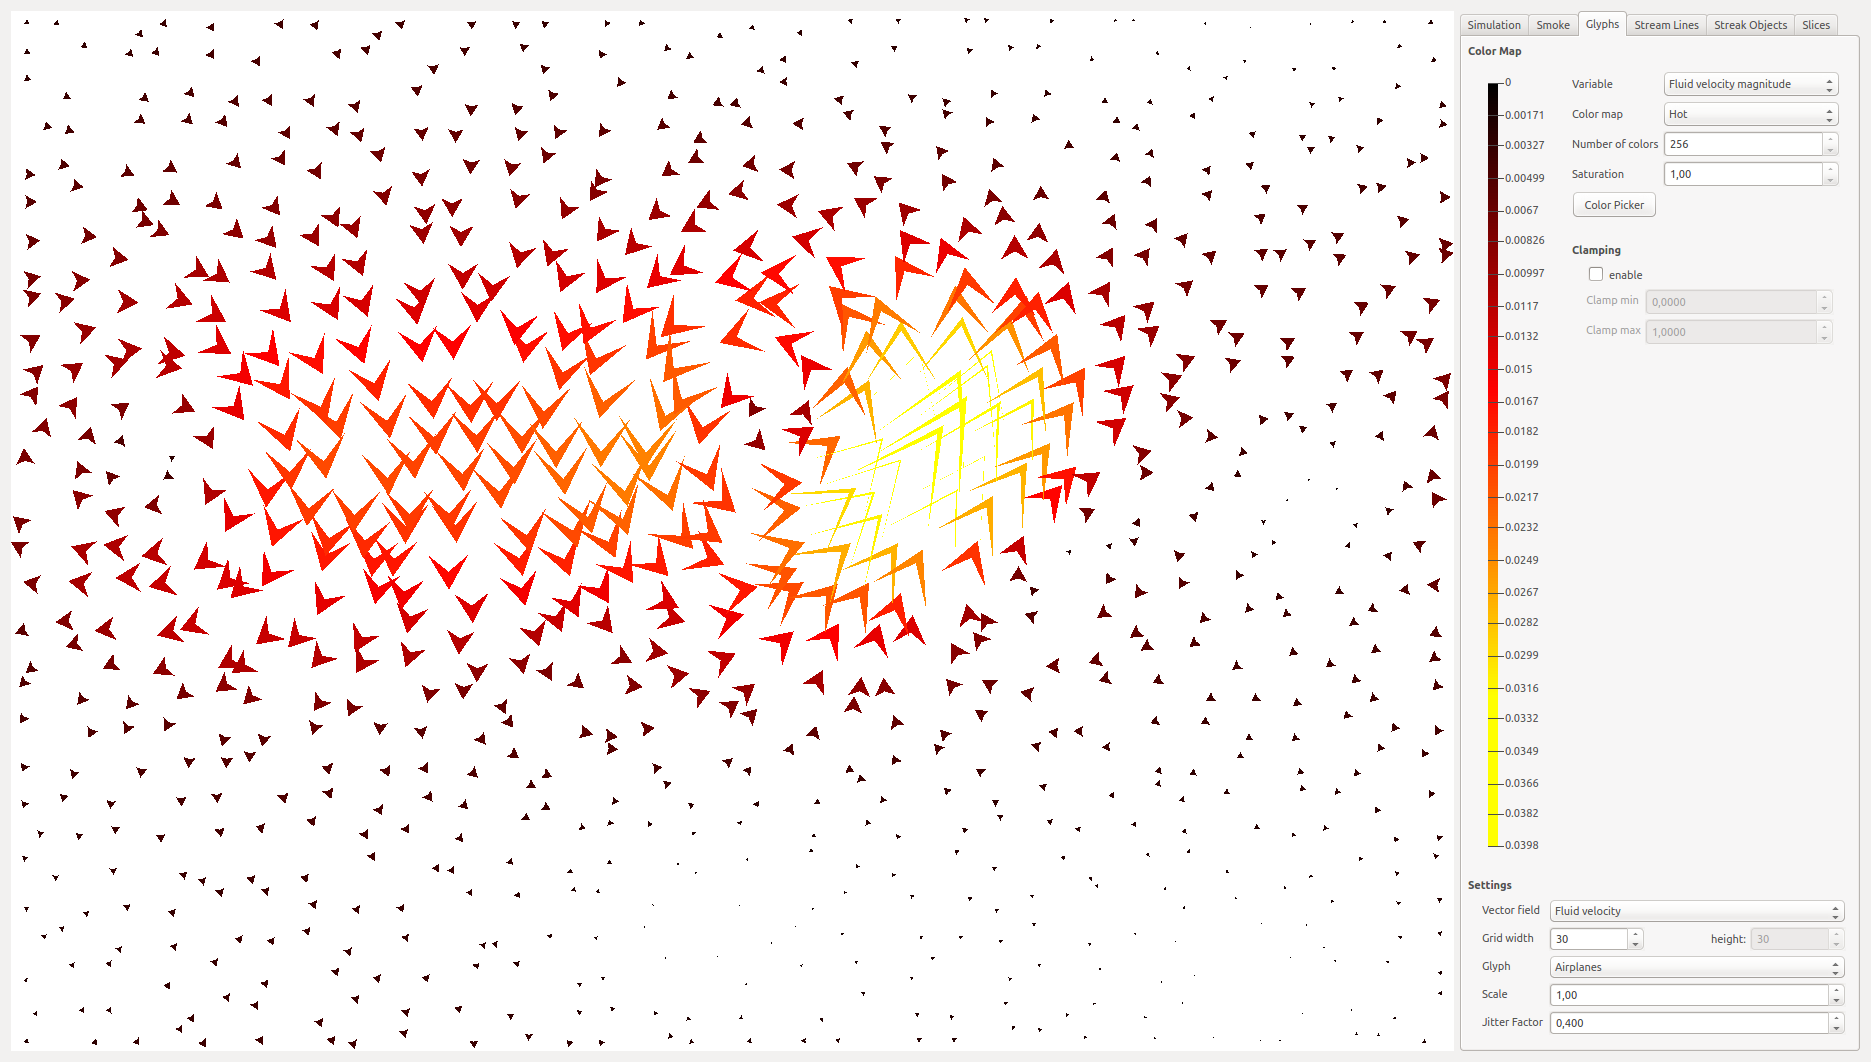
\includegraphics[width=\textwidth, trim={35px 30px 430px 30px},clip]{img/glyphs/airplanes.png}
		\caption{Example of hedgehogs showing the fluid velocity on a 30x30 grid.}
		\label{fig:glyphs:airplanes}
	\end{subfigure}
	\caption{Three visualization on the same simulation showing fluid velocity using hedgehogs, triangles, and airplane glyphs.}
	\label{fig:glyphs}
\end{figure}

Looking at the various glyphs in \cref{fig:glyphs} we can make the following observations about the glyphs.
\begin{itemize}
	\item The hedgehog glyphs shown in \cref{fig:glyphs:hedgehogs} are able to show the general flow of the fluid velocity. A disadvantage of the hedgehog is that it is hard to see the size of an individual hedgehog, making it harder to use its magnitude for the inverse mapping to the fluid velocity. Furthermore is it not possible to distinguish sources and sinks since the glyphs do not have a clear origin and destination.
	\item The triangle glyphs in \cref{fig:glyphs:triangles} are able to show the direction of the vector field more clearly. There is also a clear distinction between glyphs with a large and a small magnitude. We can also see the two disadvantages mentioned in \cref{sub:triangles}. When the magnitude of the glyph is near zero the triangles appear as lines and when its magnitude is around its max the triangle becomes nearly equilateral making it harder to see the direction in which it is pointing.
	\item The airplane glyph is shown in \cref{fig:glyphs:airplanes}. Here we can see that the glyph can display direction pretty well and put a larger emphasis on the direction of glyphs with a larger magnitude. We can also see the disadvantage discussed in \cref{sub:airplanes}, when the glyphs become too large the `wings' of the airplane appear very thin making the glyph harder to see.
\end{itemize}

In general we can conclude that although glyphs provide a nice way to visualize vector data the method also has many problems. The glyphs require space to be drawn, can occlude each other, sampling artifacts can appear, and directions are sometimes hard to decode. Some of these problems are partly solved by adding jitter to the grid and by using different types of glyphs, but most can not be solved entirely. In \cref{cha:streamlines} an alternative visualization method is given involving streamlines.


% section results (end)
